\chapter{Business Processes}
In this chapter we analyze a set of business processes which are
fundamental activities inside our organization, we provide an analysis of
these processes and the results of a simulation.

Before going in deeper details in analyzing the processes is useful to get
a wider view on the organization structure.
AllSpark, is an enterprise with the aim to develop and deploy services in
the IT area.

Our products can vary from a common web hosting service to very complex and
possibly innovative security systems, and therefore we need to distinguish
the different departments in which our organization is divided.

\section{Departments and structure}
AllSpark organization is divided in several activity areas, each one of them
contains the processes and the people needed to operate in a specific
field. 

For a more detailed view on the organization is useful to provide a
formalization of these concepts, through a set of diagrams which are going
to be described in the following sections. In particular the attention has
been focused in representing the two sides of the organization: first it's
possible to analyze which are the different roles inside the company and
how they are distributed, then is presented a view on which business
processes are involved in the different areas of the company.

\subsection{Working structure}
The working structure represent the general structure of AllSpark internal
organization. For simplicity the number of employees is not represented
since there may be several entities for each "Performer" depending on the
working load and on the size of the projects involved. Each performer is a
facet entity since several people may collaborate in that position to reach
the Roles defined, but identifying all of them with a single term and
element in the structure, permits a simpler representation of the concept.

The two main areas, Administrative and Research and Development, distinguish
the scope the employee would reach. In the former the main interest is
directly connected to the set of functions which permits the right and
complete Company lifecycle. The latter is bind to the Company productivity,
that are the basic elements which are involved in the growing of
the invoice.

The Working Team is an abstract organizational unit which represent a group
of employee which are involved in a particular project, or in some some
cases in different ones, that need different skills and knowledges to be
developed. In the organization there may be several Working Team in order to
maximize the performance in productivity and in the Project management.

The Public Relation organizational unit aims to represent the group of
people who are charged to represent the Company in meetings, in the
approaching with customers and for consulting.

Figure \ref{2img:working} can describe in details how people working for
AllSpark is organized inside the company.

\begin{figure}
\begin{centering}
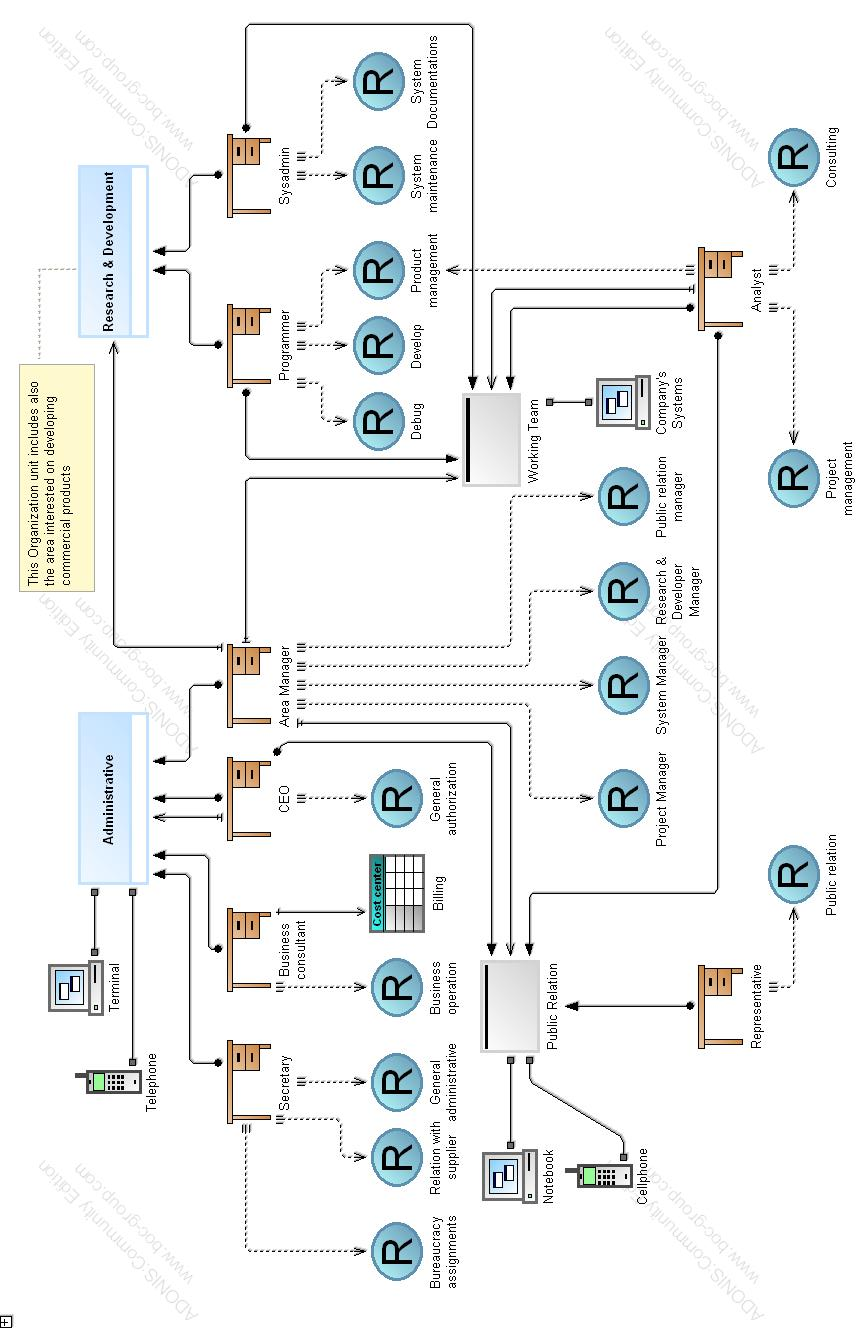
\includegraphics[scale=0.45]{assign2/adonis/imgs/working_structure.jpg}
\caption{AllSpark working structure}
\label{2img:working}
\end{centering}
\end{figure}

\subsection{Company organization}
In the AllSpark organization is possible to identify the following
different areas:
\begin{description}
\item[Administration:] This part of the enterprise manages the
administrative part of the organization, takes marketing decision, follows
the public relations with external partners, solves bureaucratic issues
and is responsible for the financial operations.
\item[Project Management:] This segment of the organization is involved in
the core processes of manage the different phases of project development.
These activities represent a set of core functions in the organizations
aims, is this sector, in facts, which is responsible for the actual
implementation of our products.
\item[Working resource management:] The processes and resources which are
involved in this sector provide support for the maintenance of hardware
and software. There are processes dedicated to reparation as to the update
of different resources.
\item[Course and Certification:] AllSpark, as an enterprise, organizes
courses for developers and sysadmins. For this reason a particular division
of the organization is dedicated to the management of courses and seminars.
\item[Research and Development:] The employees in this area work actively in
the research's world, mainly in security related field. In our organization
this section is vital for improving our products and develop new one.
\end{description}

The company map in figure \ref{2img:cmap} depicts clearly the business processes
performed in each section and how them are related to each other.

\begin{figure}
\begin{centering}
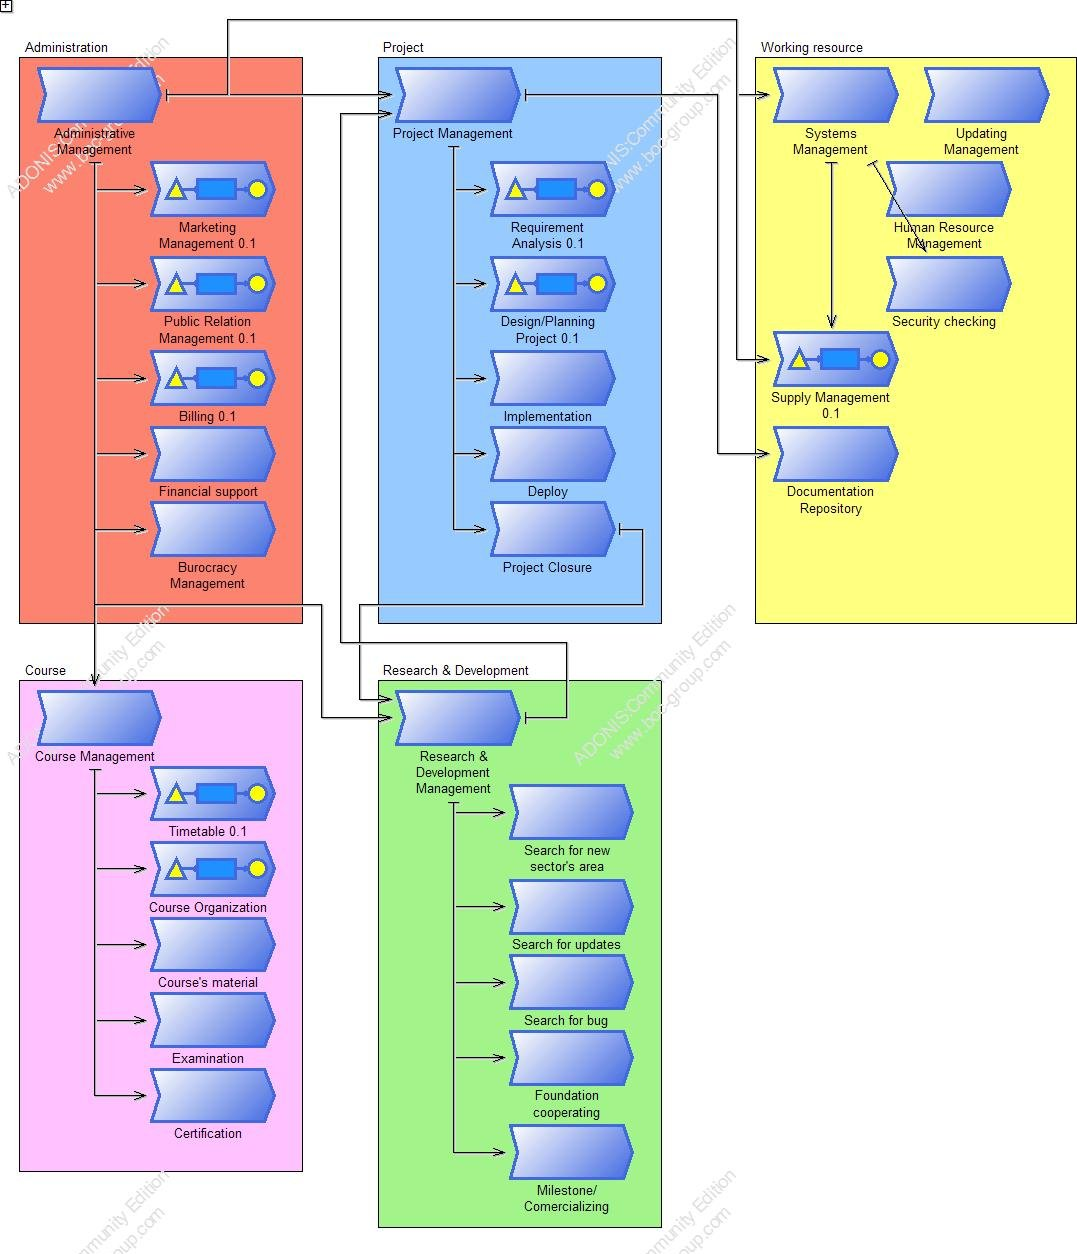
\includegraphics[scale=0.43]{assign2/adonis/imgs/companymap.jpg}
\caption{AllSpark company map}
\label{2img:cmap}
\end{centering}
\end{figure}

